% ======================================================================
% QIJ — WSOM+2026 submission
% Notation: psi = influence function; RF = receptive field (n_j counts,
% p_j = n_j/N); W = prototypes; V_tot = V_btw + V_win (identity, eq. 4).
% Figures: f3.pdf f2.pdf f7.pdf f9.pdf alongside this file.
% REVISION COPY (paper/revision/): see REVISION_PLAN.md. Original kept as qij_wsom_original.tex.
% 19 Sept 2026: rewritten to revision 8 (qij/spec/QIJ_method_spec.md). Numbers in \pending{} wait on the final run.
% ======================================================================
\documentclass[runningheads]{llncs}

\usepackage[T1]{fontenc}
\usepackage{graphicx}
\usepackage{amsmath,amssymb}
\usepackage{mathtools}
\usepackage{url}
\usepackage{booktabs}
\usepackage{xcolor}

% --- revision markup ---
% \rev{...} marks text written or rewritten for the revision: bold blue.
% Set \revfalse before the final build to print revised text plainly.
\newif\ifrev \revtrue
\newcommand{\rev}[1]{\ifrev{\color{blue}\bfseries #1}\else#1\fi}
% \pending{...} marks a number or figure that waits on the final run; none may survive to submission.
\newcommand{\pending}[1]{{\color{red}[#1]}}

% --- notation ---
\newcommand{\ifl}{\psi}
\newcommand{\Vcell}{V_{\mathrm{btw}}}
\newcommand{\Vwithin}{V_{\mathrm{win}}}
\newcommand{\Vtotal}{V_{\mathrm{tot}}}
\newcommand{\Fhat}{\hat F}
\newcommand{\Vwinhat}{\hat V_{\mathrm{win}}}
\newcommand{\Vtothat}{\hat V_{\mathrm{tot}}}
\newcommand{\XVQ}{\ensuremath{\mathcal{X}}-VQ}
\newcommand{\IVQ}{\ensuremath{\mathcal{I}}-VQ}
\newcommand{\MX}{M_{\mathcal{X}}}
\newcommand{\MI}{M_{\mathcal{I}}}
\newcommand{\psinull}{\hat{\psi}_0}
\newcommand{\psih}{\hat{\psi}}
\newcommand{\Bhat}{\hat{B}}
\newcommand{\hqij}[1]{h^{\mathrm{QIJ}}_{#1}}
\newcommand{\hboot}[1]{h^{\mathrm{boot}}_{#1}}

\begin{document}

\title{Vector Quantization for Uncertainty Quantification: The Quantized Infinitesimal Jackknife}

\titlerunning{Vector Quantization for Uncertainty Quantification}
% ORCID iDs can be added via \orcidID{...} after each name if desired
\author{Josh Taylor\inst{1}\thanks{Corresponding author.} \and
Stella S. R. Offner\inst{1}}
\authorrunning{J. Taylor and S. S. R. Offner}
\institute{The University of Texas at Austin, Department of Astronomy and Oden Institute for Computational Engineering and Sciences, Austin, Texas, USA
\email{joshtaylor@utexas.edu}}

\maketitle

\begin{abstract}
\rev{Nonparametric confidence intervals for an estimate $\hat T$ are usually obtained by the bootstrap: recompute the estimator on $B$ resampled datasets and read the interval from the replicates. The cost is $B$ evaluations of the estimator, which is prohibitive when one evaluation is an optimization. We show that a vector quantizer fitted to the data gives a much cheaper route to the same interval when the estimator's influence function has no closed form. The Quantized Infinitesimal Jackknife (QIJ) works in two stages. A quantizer of the data supplies a rough estimate of the influence function from a few hundred evaluations on the prototypes. A second, one-dimensional quantizer groups the data by that estimate into bins inside which the influence varies little, and the estimator is differenced along each bin's mass on the full data. Propagating the known multinomial fluctuation of the bin masses through these differences gives the variance and skewness of the sampling distribution, and a BCa-form interval. Nothing is resampled. On two synthetic distributions (Pareto; multivariate $t$ in ten dimensions) and two astronomical datasets (the galaxy Fundamental Plane; a stellar initial mass function fitted by constrained maximum likelihood), QIJ's interval matches the bootstrap's coverage and width on \pending{eleven of thirteen} estimands at \pending{a third or less} of the bootstrap's computation, and reports the share of the variance it measured directly on every estimand.}
\keywords{vector quantization \and uncertainty quantification \and confidence intervals \and influence functions \and bootstrap}
\end{abstract}


% ======================================================================
\section{Introduction}\label{sec:intro}
% ======================================================================

Vector quantization (VQ) compresses a dataset $X = \{x_i \in \mathbb{R}^d\}_{i=1}^N$ into $M \ll N$ prototypes $W = \{w_j\}_{j=1}^M$ to facilitate signal encoding, clustering, density representation \cite{graf2000}, and, through self-organizing maps and their descendants, topology-preserving visualizations. In this work, we assign VQ the task of constructing confidence intervals for an arbitrary parameter estimate  computed from $X$.

The bootstrap \cite{efron1979} is the gold standard for nonparametric interval estimation: recompute the estimator $T$ on $B$ resampled datasets, with $B$ in the hundreds to thousands, and infer CIs from the replicated sampling distribution of $T$. When a single evaluation of $T$ is expensive, e.g., the result of an optimizer-based fit, a profile likelihood, or an ensemble fit, those $B$ evaluations dominate the analysis. Since a VQ represents a large dataset compactly, one might expect its prototypes to stand in for the $N$ sample points during resampling; this works well for point estimates, but not for interval estimation. That is, in terms of uncertainty quantification, the quantizer prototypes are not just a smaller dataset from which to resample. Quantization suppresses precisely the sampling noise that interval estimation requires. We can, however, recover a notion of sampling variability by studying how resampling variance interacts with a VQ partition: there is variation in \emph{how many} points land in each region, and also in \emph{which} points represent each region. The VQ objective minimizes the second part by construction (if the VQ is trained properly); in this work we exploit multinomial models of the first to obtain CIs.

To achieve this, we replace explicit resampling with perturbation. Under bootstrap resampling, the counts $(n_1,\dots,n_M)$ of data in each region fluctuate acording to a multinomial covariance. Importantly, no simulation is required to learn it. The only unknown is how sensitive the estimator is to each changing count, and that is a derivative: perturb one region's share of the data, re-evaluate $T$, and record the response. Our Quantized Infinitesimal Jackknife (QIJ) does exactly this, via $\mathcal{O}(M)$ deterministic evaluations of $T$ in total, and propagates the counts' known covariance through these responses (the delta method), yielding the variance and skewness of $T$'s sampling distribution. The result is a VQ-based confidence interval with no resampling at any stage (Sect.~\ref{sec:method}).

\rev{The perturbation route needs one thing the quantizer does not provide: bins inside which the estimator's influence is nearly constant. The variance of an estimator splits into the part explained by how many points land in each bin and the part left by which points those are. Perturbing bin masses measures the first part exactly. Nothing measured along bin masses can recover the second, because the average response of a bin says nothing about the spread inside it. With bins that are the quantizer's own receptive fields, the second part is small only where the influence happens to be flat inside each cell, and on the multivariate $t$ and Fundamental Plane estimators of Sect.~\ref{sec:results} it is more than half of the variance. The bins must therefore follow the influence, and the influence is what we do not know.}

\rev{The observation that makes this possible is that the influence function is a derivative of the estimator, and a derivative can be taken on a coarse version of the data. Evaluating the estimator on the quantizer's prototypes as a weighted dataset, and again with each prototype's weight nudged, gives an estimate of the influence at every prototype from a few hundred cheap evaluations. A smooth model through those values gives an estimate at every data point. Grouping the data by that estimate gives bins that follow the influence before any full-data evaluation is spent. The finite differences on the full data then measure the between-bin part, and the same differences say where the grouping was too coarse and should be refined. What remains inside the bins is predicted from the model, and the two parts add up to the variance estimate. The decomposition is an algebraic identity on any partition (Sect.~\ref{sec:identity}), and it is what lets us report how much of the variance was measured and how much was predicted.}

\paragraph{Related work.} The infinitesimal jackknife originates with Jaeckel \cite{jaeckel1972}; Efron \cite{efron1982} connects it to the bootstrap. Wager et al.\ \cite{wager2014}, similarly motivated by an estimator too expensive to resample, apply it to random forests, though their derivative is taken with respect to individual observation weights, whereas ours is taken with respect to Voronoi masses. The Bag of Little Bootstraps \cite{kleiner2014} and $m$-out-of-$n$ subsampling \cite{bickel1997} reduce the size of each resample but still resample, and their approximation error is asymptotic and unobserved; QIJ never resamples, and its approximation error is a reported quantity. The influence-function machinery we rely on is classical robust statistics \cite{hampel1974,stefanski2002}. \rev{Influence functions computed by differentiating a fitted model, rather than resampling it, are used in machine learning to trace a prediction back to training points \cite{koh2017} and to approximate cross-validation \cite{giordano2019}; both need the model's Hessian, which we do not have. The ABC intervals of DiCiccio and Efron \cite{diciccio1996} build BCa-form intervals from analytic derivatives of the estimator, which is where our interval's form comes from. Coresets \cite{feldman2011} compress a dataset so that a fit on the summary approximates the fit on the data; our prototype stage uses the summary for a derivative, not a fit, and the two need not agree in value. Learning vector quantization with an adapted metric \cite{hammer2002,schneider2009} bends the quantizer toward the quantity of interest, which is what our second quantizer does with the influence itself; and quantizing by an estimated gradient rather than by position is the idea behind gradient-based dimension reduction \cite{xia2002}.}

% ======================================================================
\section{The Quantized Infinitesimal Jackknife}\label{sec:method}
% ======================================================================

\subsection{Setup: Influence Functions and Bin Influences}\label{sec:setup}

Let $X=\{x_i\}_{i=1}^{N}$ be iid from $F$, let $\hat{F}$ be its empirical
distribution, and let $T$ be a functional on distributions, so that the
estimand is $\theta = T(F)$ and the estimator is its plug-in
$\hat{T} = T(\hat{F})$. The influence function of $T$ at $\hat{F}$ is
%
\begin{equation}\label{eq:if}
  \psi(x) \;=\; \lim_{\varepsilon \to 0}
  \frac{T\!\big((1-\varepsilon)\hat{F} + \varepsilon\,\delta_x\big) - T(\hat{F})}
       {\varepsilon},
\end{equation}
%
the derivative of $T$ in the direction of a point mass at $x$, i.e.\ how much
the estimate moves per unit of probability placed at $x$; it satisfies
$\sum_i \psi(x_i) = 0$. The classical linearization
$\hat{T} - \theta \approx \tfrac{1}{N}\sum_i \psi(x_i)$~\cite{vonmises1947,hampel1974}
underlies both the jackknife and the bootstrap, and gives
$\operatorname{Var}(\hat{T}) \approx \mathbb{E}[\psi^2]/N$.

\rev{Two vector quantizers appear below. The \XVQ{} quantizes the data: its prototypes are $w_j$, each with a receptive field $\mathrm{RF}_j$ of $n_j$ points and mass $p_j = n_j/N$. The \IVQ{} quantizes an estimate of the influence itself, and its cells, which we call bins, are indexed by $k$. The construction that follows applies to any set $K$ of data points, receptive field or bin.} The influence of a set $K$ with $n_K$ points is the derivative of $T$ with the point mass replaced by an equal spread of mass over the points of $K$:
%
\begin{equation}\label{eq:Uj}
  U_K \;=\; \lim_{\varepsilon \to 0}
  \frac{T\!\Big((1-\varepsilon)\hat{F}
        + \frac{\varepsilon}{n_K}\sum_{i \in K} \delta_{x_i}\Big)
        - T(\hat{F})}{\varepsilon}
  \;=\; \frac{1}{n_K} \sum_{i \in K} \psi(x_i).
\end{equation}
%
The perturbation raises the set's mass by $\varepsilon$ at the expense of the
others, reweighting every point inside it identically (never individually).
Since the derivative is linear in the direction perturbed, the response is the
average of the individual responses $\psi(x_i)$, which is the second equality. \rev{For a bin we write $U_k$ and call it the bin influence.}

Eq.~\eqref{eq:Uj} is the infinitesimal jackknife (IJ) of~\cite{jaeckel1972} with its perturbation space restricted to the masses of $M$ sets instead of $N$ observation weights. At $M = N$ each set holds a single point and $U_K = \psi(x_K)$; at $M = 1$ the single set gives $U = 0$. \rev{When $\psi$ has a closed form, the $U_K$ are averages of known numbers. This paper is about the other case, in which $T$ is available only as a program: one \emph{estimator evaluation} is a call $T(X,\omega)$ on the data with non-negative weights $\omega$ summing to $N$, and $U_K$ is obtained by finite differences of that call (Sect.~\ref{sec:difference}).}

The counts obtained under resampling are jointly multinomial: redistributing $N$ draws into a fixed partition gives $\mathrm{Cov}(n_k, n_l) = N(p_k \delta_{kl} - p_k p_l)$, with no simulation required to learn this covariance structure. Propagating this known fluctuation through the derivatives via the delta method gives the variance estimate
\begin{equation}\label{eq:Vcell}
\Vcell \;=\; \frac1N \sum_{k=1}^{M} p_k\, U_k^{2},
\end{equation}
using the fact that $\sum_k p_k U_k = 0$. The same quantities supply the third moment of the influence distribution, from which the skewness correction of the BCa interval \cite{efron1987} follows with no additional evaluations; the median-bias constant $z_0$, conventionally taken from bootstrap replicates, is set to zero.

\subsection{The Variance Decomposition}\label{sec:identity}

With $U_k$ as above and $\mathrm{Var}_k(\ifl) = \tfrac{1}{n_k}\sum_{i \in k}(\ifl(x_i) - U_k)^2$ the spread of influence among the points inside bin $k$,
\begin{equation}\label{eq:identity}
\underbrace{\frac1N\sum_{i=1}^{N} \ifl(x_i)^{2}}_{N\,\Vtotal}
\;=\;
\underbrace{\sum_{k=1}^{M} p_k\, U_k^{2}}_{N\,\Vcell}
\;+\;
\underbrace{\sum_{k=1}^{M} p_k\, \mathrm{Var}_k(\ifl)}_{N\,\Vwithin}.
\end{equation}
This is the between/within variance decomposition applied to the influence values, and it holds \emph{algebraically} on any dataset and any partition. The left side contains no partition information, while both right-side terms depend on it strongly. \rev{The identity also states the obstacle that shapes the rest of the method. The bin influences $U_k$, however exactly they are obtained, say nothing about $\Vwithin$: averages over a set of points do not determine the spread inside the set. With bins that are the receptive fields of the \XVQ, $\Vwithin$ is small only where $\psi$ happens to vary little inside each Voronoi cell; on the multivariate $t$ and Fundamental Plane estimands of Sect.~\ref{sec:results}, receptive fields at $M = 40$--$50$ leave 54--80\% of the variance inside them, and no number of evaluations along their masses can recover it. Without a closed form for $\psi$, the only route is to build bins inside which $\psi$ is nearly constant, which requires knowing its shape before the finite differences are taken. The \XVQ{} supplies that shape cheaply (Sect.~\ref{sec:xvq}) and the \IVQ{} then makes $\Vcell$ nearly the whole of $\Vtotal$ (Sect.~\ref{sec:ivq}).}

\subsection{Finite Differences Along a Bin's Mass}\label{sec:difference}

\rev{Let $K$ be a bin with mass $p$. Raising its mass by a fraction $\delta$ of itself and lowering every other point's weight in proportion gives weights $\omega_i = (1-t) + t\,\mathbf{1}\{i \in K\}/p$ with $t = \delta p/(1-p)$; they sum to $N$, every weight stays non-negative for $\delta \le 1$, and the direction is the multinomial one of \eqref{eq:Vcell}. Write $T(t)$ for the estimator at these weights, with $T(0) = \hat T$ shared by every bin, and define $U_K$ as the derivative with respect to $t$. The step is a fraction of the bin's own mass rather than a fixed amount of mass, so that a small bin is not perturbed proportionally more than a large one; with a fixed absolute step, a bin holding one percent of the data has its mass more than doubled, and the difference is a chord across a large change rather than a derivative. The derivative carries a truncation error from the step and a rounding error from the estimator's accuracy $\eta$, the relative size of the part of one evaluation that does not reproduce. Balancing the two gives $\delta = (3\eta)^{1/3}$ for the central stencil $U_K = [T(t) - T(-t)]/(2t)$, which also yields the second difference $\Delta^2 T_K = [T(t) - 2T(0) + T(-t)]/t^2$, and $\delta_f = 2\sqrt{\eta}$ for a single forward step $U_K = [T(t) - T(0)]/t$. The user declares $\eta$: machine precision for a closed form, the solver's tolerance for an iterative estimator.}

\subsection{The $\mathcal{X}$-VQ and the Initial Influence Estimate}\label{sec:xvq}

\rev{The shape of $\psi$ can be learned cheaply because $\psi$ is a derivative of $T$, and derivatives can be taken on a coarse version of the data. Fit the \XVQ{} with $\MX$ prototypes ($k$-means centroids; $\MX$ is set below) to the data in whitened coordinates. Evaluate $T$ on the prototypes as a weighted dataset of $\MX$ rows, each prototype carrying its mass, and then once more per prototype with that prototype's mass raised by the fraction $\delta_f$ and the others lowered in proportion. The differences, mass-centred, are the \emph{prototype influences} $I_j$: the derivative of $T$ at the quantized data along prototype $j$'s mass. They are influence values of the quantized distribution, not of the data, and the two can differ in scale. Centroids thin the tails of a distribution, so on the multivariate $t$ the estimator returns a degrees-of-freedom value of about \pending{150} on the prototypes against $5.6$ on the full data of the same draw. What the next stage needs from the $I_j$ is their level structure, which points are high and which are low, and Fig.~\ref{fig:influence} reports how well that structure agreed with the true influence. The cost is $1 + \MX$ evaluations on $\MX$ rows.}

\rev{A Gaussian process with an affine mean and a Mat\'ern-$3/2$ kernel is passed through the pairs $(w_j, I_j)$ \cite{rasmussen2006}. Its width and the ratio of its noise to its signal variance are set by maximum marginal likelihood, with the noise ratio profiled at each width, and the smallest width allowed equal to the median distance between prototypes that the \XVQ's connectivity graph joins. The prototype influences carry evaluation noise: each is a difference of two evaluations of accuracy $\eta$ divided by a step $t_j$, so its noise has standard deviation about $\sqrt{2}\,\eta\,|T|/t_j$. Left free, the likelihood on a noisy estimator drives the noise ratio to zero and interpolates that noise as signal, and the model then reports the resulting wiggle as variation inside the bins. The noise ratio is therefore not allowed below the level the declared $\eta$ implies. For a closed-form estimator that level is far below the search's floor and nothing changes; for the optimizer-based estimator of Sect.~\ref{sec:data} it is what makes the model's uncertainty honest. The posterior mean at a data point is the \emph{initial influence estimate} $\psinull(x_i)$, and the posterior standard deviation is its uncertainty $\sigma_i$, small where prototypes are dense and large in the tails. The affine mean matters: a zero-mean kernel model returns to zero beyond the outermost prototype, and on heavy-tailed data the most influential points lie exactly there. No estimator evaluations are spent here.}

\rev{\paragraph{How many prototypes.} The first stage costs about $\MX^2$ rows of evaluation and the finite differences of the second about $(1 + 2q\,M_{\mathrm{ref}})N$ rows for $q$ outputs, with $M_{\mathrm{ref}}$ the bin count of Sect.~\ref{sec:ivq}. We give the \XVQ{} the same row budget as the finite differences it serves,
\begin{equation}\label{eq:MX}
\MX \;=\; \Big\lceil \sqrt{(1 + 2q\,M_{\mathrm{ref}})\,N/2}\,\Big\rceil,
\end{equation}
floor 20, cap $N/2$: $188$ prototypes for a one-output estimator at $N = 2000$, $371$ for the four-output Fundamental Plane and $414$ for the five-output initial mass function. This is a budget rule, not an accuracy rule. No rule known before running guarantees that the prototypes resolve an unseen estimator's influence; Sect.~\ref{sec:res-limits} tests this on a tail probability in ten dimensions. The cost of the whole method is known before running, about twice the finite differences, against $BN$ rows for the bootstrap; the diagnostics of Sect.~\ref{sec:outputs} say afterwards whether the \XVQ{} was fine enough.}

\subsection{The $\mathcal{I}$-VQ and Gain-Driven Refinement}\label{sec:ivq}

\rev{Evaluate $T$ on the full data once. Then quantize the values $\psinull(x_i)$ with a one-dimensional $k$-means into $\MI$ bins, each the set of data points whose initial influence estimate falls in one interval. For an optimal one-dimensional quantizer with $M$ levels the share of the variance left inside the bins is about $\kappa/M^2$ \cite{panter1951,graf2000}, with $\kappa = 2.7$ for normally distributed values, so a declared tolerance $\epsilon$ on that share gives $M_{\mathrm{ref}} = \lceil\sqrt{2.7/\epsilon}\,\rceil$, $17$ at $\epsilon = 0.01$. We start at $\MI = M_{\mathrm{ref}}$ and let the finite differences decide the rest. Each initial bin is differenced with the central stencil, two evaluations on $N$ rows, giving $U_k$ and $\Delta^2 T_k$; the $U_k$ are centred so that $\sum_k p_k U_k = 0$.}

\rev{Refinement splits the bins where the finite differences say the grouping is too coarse. Every bin with more than one point carries a proposed split and an expected gain, the increase in $\Vcell$ the split would produce if $\psinull$ were right, brought to the finite-differenced scale by $\rho^2$, the ratio of $\Vcell$ to the between-bin variance of $\psinull$. The model's uncertainty inside a bin is $v_k$, the variance of its error around the error common to the bin (the common part is already fixed by $U_k$). The split is by level, a two-means on the bin's $\psinull$ values, when the estimate varies inside the bin more than $v_k$; otherwise by adjacency, separating the points whose second-nearest prototype carries a higher prototype influence than their nearest, with expected gain $\rho^2 p_k v_k/N$. The bin with the largest expected gain is split; the smaller child is differenced with one forward step and the larger follows by subtraction, since a parent's bin influence is the mass-weighted sum of its children's. The realized gain is the increase in $\Vcell$ the split actually produced. A lineage stops when its realized gain falls below the bin's share of the tolerance, $\epsilon\,\Vcell/L$ with $L$ the current number of bins; the loop stops when no expected gain exceeds that share, and at most $1 + \MX$ evaluations are spent refining. The ratio of realized to expected gains over the run is reported: it is how well $\psinull$ predicted. Refinement acts on variation that the initial estimate shows, or that the model's uncertainty inside a bin points to; Sect.~\ref{sec:res-limits} tests it on an influence that the initial estimate cannot see.}

\subsection{Outputs}\label{sec:outputs}

\rev{Three quantities follow without a model. The between-bin term $\Vcell = \frac1N\sum_k p_k U_k^2$ over the final $L$ bins is finite-differenced on the full data, is a lower bound on $\Vtotal$ exact up to the step error, and rises with every split. The bias term $\Bhat = \frac{1}{2N}\sum_k p_k \Delta^2 T_k$ is the second-order term of the expansion of $\hat T$ along the bin masses; it is reported and not applied (Sect.~\ref{sec:res-limits} says why). The BCa acceleration $\hat a_{\mathrm{BCa}}$ comes from the third moment of the refined estimate $\psih(x_i) = U_{k(i)} + \rho\,(\psinull(x_i) - \bar\psi_{0,k(i)})$. The remainder is predicted: $\Vwinhat = \rho^2\,\frac1N\sum_k p_k\,\gamma_k\,[\mathrm{Var}_k(\psinull) + v_k]$ over bins with more than one point, where $\gamma_k \le 1$ is the realized fraction of the expected gain in the split that created the bin, so that a bin whose split showed the model's variation to be spurious is discounted, and $\gamma_k = 1$ for a bin never split. $\Vtothat = \Vcell + \Vwinhat$ is the variance estimate. The QIJ interval at level $q$, $\hqij{q}$, is the BCa-form interval with variance $\Vtothat$, acceleration $\hat a_{\mathrm{BCa}}$, median-bias constant zero and centre $\hat T$. Reported alongside: evaluation counts by size, rows processed normalized by $N$, wall time, $L$ and the split counts, $\rho$, the ratio of realized to expected gains, and the kernel width and noise ratio with a note when either sits on a bound.}

\subsection{Scope}\label{sec:scope}

\rev{Five conditions bound the method. The estimator must accept a weighted point set and be well defined on coarse weighted data within the data's range. An evaluation that fails, or that ends on a bound of the estimator's parameter box, returns no value; the method counts it, uses the same rule for a bootstrap replicate, and never retries. A prototype whose evaluation failed is left out of the influence model; a failed evaluation of an initial bin, or a prototype stage on which every prototype responds alike, fails the draw, and the paper reports how often that happened. An estimator that is not differentiable in the weights (a quantile, a hard threshold, model selection inside $T$) is out of scope, as for every influence-based method. An estimator whose influence is discontinuous in $x$, such as a tail probability, is in scope, with any loss reported: the prototype stage sees a jump only where a prototype sits on its far side, and a data point whose influence differs from its neighbours' while its prototype's centroid sits with the neighbours is invisible to the initial estimate. Whether the refinement recovers such a point depends on the model's uncertainty marking its bin; where it does not, $\Vcell$ stays a lower bound short of $\Vtotal$ by that point's share and the interval under-covers by the same share (Sect.~\ref{sec:res-limits}). The value of $T$ at the quantized data is the functional at that distribution and is never reported as an estimate of $\theta$. The accuracy $\eta$ is the user's declaration and is not checked. The multinomial covariance in \eqref{eq:Vcell} assumes iid sampling.}

\begin{figure}[t]
\centering
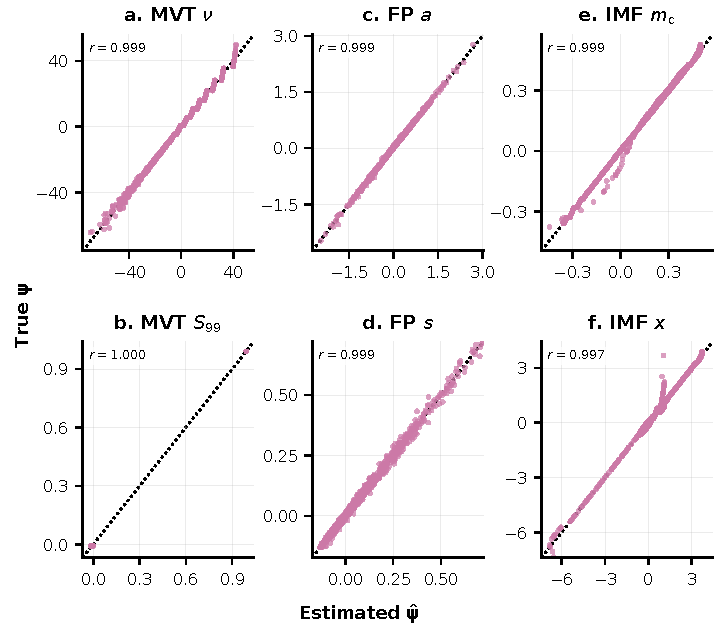
\includegraphics{fig_b.pdf}
\caption{\rev{The refined influence estimate against the true influence on one draw ($N = 2000$), one point per prototype of the \XVQ: the true influence averaged over the prototype's receptive field (hollow) and the refined estimate $\psih$ averaged over the same field (filled), against the receptive field's mean position on one data axis. Printed in each panel: the rank correlation between the two series and $\rho$. (a, b) multivariate $t$, $\nu$ and the tail probability, against radius; (c, d) Fundamental Plane, coefficient $a$ and the scatter, against $\log\sigma$; (e, f) initial mass function, slope and cutoff sharpness, against $\log$ stellar mass. \pending{Figure and per-panel numbers from the final run.}}}
\label{fig:influence}
\end{figure}

% ======================================================================
\section{Experimental Data}\label{sec:data}
% ======================================================================

We evaluate QIJ on \rev{four datasets. Two are from distributional families in which the ground truth is known; two are astronomical, with vector-valued estimands, and one of those is fitted by a constrained optimizer. Each estimator has an analytic influence function, which QIJ never sees: every estimator enters the method as a program that returns a value for a weighted dataset, and the closed form is used only to judge the result. From each data process, $S = 1000$ Monte Carlo draws of size $N = 2000$ were taken. QIJ and the nonparametric bootstrap ($B = 2000$ replicates) were run on identical draws paired by seed. QIJ's declared inputs were $\epsilon = 0.01$ throughout, and $\eta$ at machine precision for the closed-form estimators, $10^{-12}$ for the two solved by a root-find or an eigendecomposition, and $10^{-6}$ for the initial mass function, the square root of its optimizer's tolerance. The rule \eqref{eq:MX} then gave $188$ prototypes for each one-output estimator, $371$ for the Fundamental Plane and $414$ for the initial mass function; every output started from $17$ bins, and Table~\ref{tab:t1} reports where refinement ended. Nothing was tuned per dataset.} The astronomical cases use an empirical population protocol: a large catalogue is treated as the population, draws are sampled from it with replacement, and the target $\theta_{\mathrm{true}}$ is the parameter vector computed from the full catalogue. Below, we describe the datasets individually.

\paragraph{Pareto.} A heavy-tailed distribution, with closed-form influence functions for both estimators (the shape parameter's maximum-likelihood estimator, and a tail probability), so every stage of the pipeline can be checked analytically. \rev{The shape parameter's influence is unbounded in $\log x$, which makes the tail beyond the outermost prototype the test of the initial estimate; the tail probability's influence is a step in one dimension, which the initial bins separate on their own.}

\paragraph{Multivariate $t$ (MVT).} A ten-dimensional, elliptically symmetric distribution with two estimands: the degrees of freedom $\nu$ (estimated by profile maximum likelihood), and the probability of the one-percent tail beyond a fixed radius. This tests whether our construction survives higher data dimension. \rev{The $\nu$ estimator is the case in which the quantized data are far from the data: centroids thin the tails, and on the prototypes the estimator returns a $\nu$ in the hundreds for a $\nu = 5$ sample. The tail probability is the hard case: its influence is a step across a sphere in ten dimensions, and only about twenty of the $2000$ points lie beyond it.}

\paragraph{Galaxy fundamental plane.} The galaxy Fundamental Plane dataset (FP) comprises 76{,}997 early-type galaxies drawn from the Sloan Digital Sky Survey Data Release 7 spectroscopic catalog \cite{abazajian2009}. For each galaxy, the three Fundamental Plane observables are the aperture-corrected stellar velocity dispersion $\sigma$ (following the correction of \cite{jorgensen1995}), the effective radius $R_e$, and a luminosity-based surface brightness proxy $I_e$. The Fundamental Plane is fit in log-space as $\log R_e = a\,\log\sigma + b\,\log I_e + c$ via least squares. The estimands are the coefficient vector $(a,b,c)$ and the intrinsic scatter about the plane. \rev{The four outputs come from one evaluation, so the Fundamental Plane is the vector case: one \XVQ{} and four \IVQ{}s, the four sharing every evaluation.}

\rev{\paragraph{Stellar initial mass function (IMF).} The population is 19{,}857 stellar masses from the STARFORGE star-formation simulations \cite{grudic2021,guszejnov2022}. The estimator fits a two-regime mass function by weighted maximum likelihood: a gamma density below a fixed split of $0.177$ solar masses, and above it a power law of slope $\alpha$ with an exponential cutoff at mass $M_*$ whose sharpness is $p$. Continuity of the density and its slope at the split fixes the gamma's shape and scale from $(\alpha, M_*, p)$, so three parameters are free and five are reported. The fit is a bounded trust-region minimization with an analytic gradient and Hessian, from one starting point computed by the method of moments from the weighted data, so that a bootstrap replicate and a QIJ evaluation are computed identically. A fit that ends on a bound of its parameter box returns no value and is counted as failed, for both methods. This is the case the method is meant for: one evaluation is an optimization, and the cutoff is identified by the few most massive stars, which a resample can lose.}

% ======================================================================
\section{Results}\label{sec:results}
% ======================================================================

\rev{Table~\ref{tab:t1} reports every estimand; Figs.~\ref{fig:accuracy}--\ref{fig:cost} show six of the thirteen, chosen to cover the four datasets and both kinds of difficulty. Every number in this section comes from the same $1000$ draws. \pending{Numbers below wait on the final run and are marked.}}

\subsection{Accuracy Against the Truth and the Bootstrap}\label{sec:res-valid}

\rev{The reference for the variance is the Monte Carlo variance of $\hat T$ over the draws, and for coverage it is $\theta_{\mathrm{true}}$. On the \pending{eleven} estimands with a smooth influence or a one-dimensional step, the between-bin term alone reaches \pending{0.98--1.00} of the oracle variance, the predicted remainder is \pending{under 4\%} of it, and the QIJ interval covers at \pending{0.944--0.953} against the bootstrap's \pending{0.943--0.958} (standard error $0.007$) with widths within \pending{3\%} of the bootstrap's (Fig.~\ref{fig:accuracy}). The ratio of realized to expected gains, the method's own report on how well the initial estimate predicted, lies between \pending{0.5 and 1.0} on these estimands. The bias term matched the known bias on the closed-form estimators (\pending{Pareto: value against exact}). Fig.~\ref{fig:influence} shows what the second stage delivers: the refined estimate $\psih$ averaged over receptive fields against the true influence averaged over the same fields, with rank correlation \pending{above 0.99} on the smooth estimands.}

\begin{figure}[t]
\centering
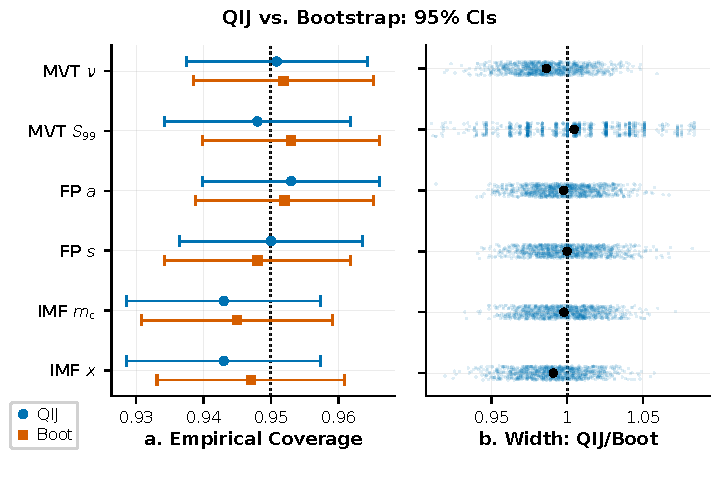
\includegraphics{fig_a.pdf}
\caption{\rev{Accuracy on the six featured estimands, rows in the order of Fig.~\ref{fig:influence}. (a) $\log$ of the variance estimate over the Monte Carlo variance of $\hat T$, for QIJ and for the bootstrap, with 95\% whiskers over draws; the band marks $\pm 0.05$. (b) Coverage at 0.95 of the QIJ and bootstrap intervals with Monte Carlo standard errors. (c) Width ratio, QIJ over bootstrap, median with the 5--95\% range; the band marks $\pm 10\%$. \pending{Figure from the final run.}}}
\label{fig:accuracy}
\end{figure}

\begin{table}[t]
\caption{\rev{All thirteen estimands: the share of the variance measured directly ($\Vcell/\Vtotal$), the variance estimate against the truth and against the bootstrap, coverage of both intervals at 0.95 (standard error $0.007$), the width ratio, the final bin count $L$, evaluations, normalized rows, the QIJ-to-bootstrap wall-time ratio within a draw, and the failed draws of each method. \pending{Table from the final run.}}}
\label{tab:t1}
\centering
\pending{T1}
\end{table}

\subsection{Where the Method Falls Short}\label{sec:res-limits}

\rev{\pending{Tail paragraph, written after the final run.} The multivariate-$t$ tail probability is the hard case. Its influence takes two values, about $-0.01$ inside a sphere and about $0.99$ beyond it, so the twenty or so points beyond the sphere carry the whole variance and each must end in a bin of its own. A point beyond the sphere whose receptive field holds two or three points inside it leaves the centroid inside, and that prototype's influence is the same as any interior one's; on the featured draw the prototype stage registered \pending{six} of the seventeen such points, and the rest are invisible to the initial estimate. What the refinement recovers of them is decided by whether the model's uncertainty inside a bin marks the bins that hold them. \pending{With the final rule the between-bin term reached the oracle exactly on one pre-flight draw and 0.87 on another; the $S = 1000$ numbers, the coverage, and the diagnostic (the ratio of realized to expected gains) go here.} At $N = 1000$ the same estimand reached the oracle exactly, because $k$-means isolated the outlying points one per prototype.}

\rev{The initial mass function's cutoff mass $M_*$ is the other shortfall: the QIJ interval covers at \pending{0.935} against the bootstrap's $0.944$. QIJ's variance for $M_*$ equals the oracle's, which is a linearization at the fitted parameters; the Monte Carlo sampling distribution of $\hat M_*$ at $N = 2000$ is \pending{11\%} wider in standard deviation and left-skewed. Both methods see a finite-sample effect the linearization does not, and the cost study of Sect.~\ref{sec:res-compute} shows it vanishing with $N$. The bias term does not help: over the draws the realized bias of $\hat M_*$ is zero within error while the bias term is heavy-tailed from draw to draw, and shifting the interval by it in either direction lowers coverage. This is why the bias term is reported and not applied. The other IMF outputs show the case the method is meant for. A quarter of bootstrap replicates lose the rare massive stars that identify the cutoff sharpness $p$ and converge to a second mode, so the bootstrap's interval for $p$ is \pending{1.5} times QIJ's at the same coverage; QIJ's evaluations never drop a point. \pending{Bound hits: bootstrap replicate fraction and QIJ evaluation fraction; failed draws of each method.}}

\subsection{Cost}\label{sec:res-compute}

\rev{Cost is reported in three forms: evaluation counts by the number of rows each processes, rows processed normalized by $N$ (one full-data evaluation equals one normalized row), and wall time. Fig.~\ref{fig:cost} shows, per featured estimand, the bootstrap's relative width error after its first $b$ replicates against $b$, and the QIJ interval at the normalized rows it spent, with the wall time of one run of each method printed in the panel. The QIJ interval costs \pending{55--70} normalized rows for a one-output estimator and \pending{277} for the four-output Fundamental Plane, against $2000$ full-data evaluations for the bootstrap; on the initial mass function, where one evaluation is an optimization, QIJ's wall time is \pending{0.29} of the bootstrap's. Fig.~\ref{fig:costN} shows the same on the Fundamental Plane as $N$ grows to the full catalogue: the bootstrap's cost grows as $BN$, QIJ's as about $N$ times the evaluations, and both intervals stay at nominal coverage. \pending{IMF panel: coverage of both intervals and the wall-time ratio against $N$, and the fraction of bootstrap replicates reaching the box against QIJ's zero.}}

\begin{figure}[t]
\centering
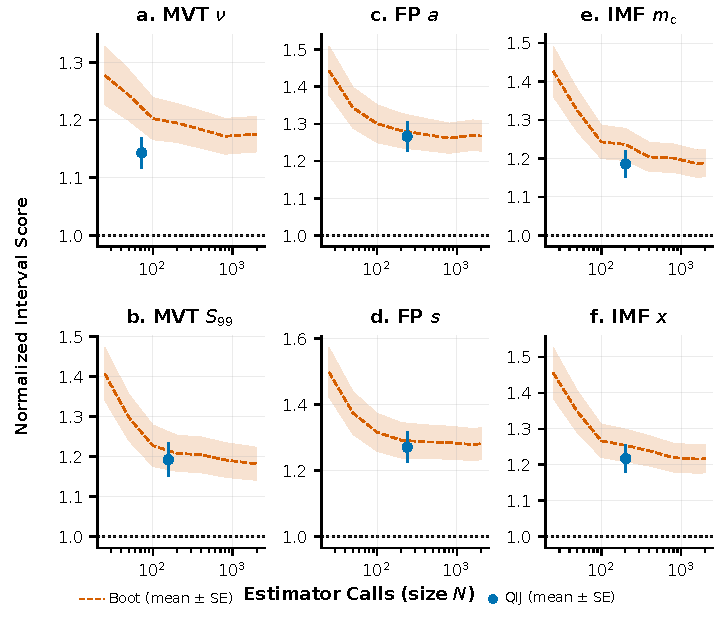
\includegraphics{fig_c.pdf}
\caption{\rev{Cost on the six featured estimands. Curve: the bootstrap's relative width error at 0.95 after the first $b$ replicates, mean over draws with the interquartile band. Marker: QIJ at its median normalized rows with interquartile whiskers, its width error against the converged bootstrap. Printed: wall time of one run of each method, one worker, one thread. Both Fundamental Plane panels print the same pair, since its four outputs come from one run. \pending{Figure from the final run.}}}
\label{fig:cost}
\end{figure}

\begin{figure}[t]
\centering
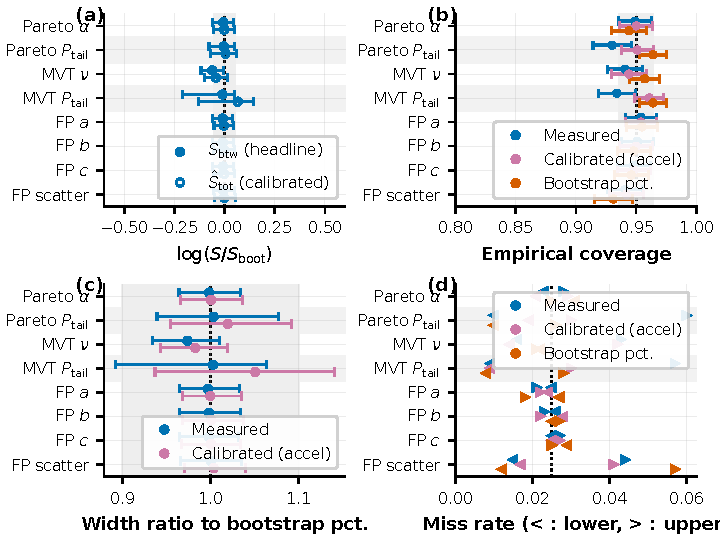
\includegraphics{fig_d.pdf}
\caption{\rev{Cost against sample size on the Fundamental Plane, $N$ from $1000$ to the full catalogue of 76{,}997 galaxies. (a) Normalized rows and wall time per run for QIJ and the bootstrap. (b) Coverage of both intervals at 0.95, one line per output with Monte Carlo bands, and the width ratio. \pending{Figure from the final run; IMF panels if run.}}}
\label{fig:costN}
\end{figure}

% ======================================================================
\section{Conclusions and Future Work}\label{sec:conclusions}
% ======================================================================

\rev{We have shown that a fitted vector quantizer supports nonparametric interval estimation for an estimator whose influence function has no closed form. The route is not resampling from the partition, which would require the sampling variability that the quantizer minimizes away, but differentiation across it. The quantizer's prototypes give a cheap estimate of the influence; a second quantizer of that estimate gives bins inside which the influence varies little; finite differences along the bin masses measure the between-bin variance on the full data, and the same differences say where to refine. The decomposition of \eqref{eq:identity} is an algebraic identity on any dataset and any partition, and it is what lets the method report how much of the variance it measured.}

\rev{On \pending{eleven} of thirteen estimands across four datasets the QIJ interval matches the bootstrap's coverage and width, at \pending{a third or less} of the bootstrap's computation, and where one evaluation is an optimization it also avoids the mode-switching that resampling causes. \pending{Shortfalls, written after the final run.} A tail probability in ten dimensions puts all of its variance on a handful of points, and a point that is not its own prototype is invisible to the initial estimate; what the refinement recovers of it is reported. A cutoff mass identified by rare stars has a finite-sample spread that a linearized variance does not see, and neither the bootstrap nor QIJ covers it at nominal at this sample size. Both are reported by the method's own diagnostics.}

\rev{The prototype count is set by a cost budget, not by accuracy, and no rule known before running can promise that the prototypes resolve an unseen estimator's influence. Two directions follow. A refinement that spends evaluations to search for variance the model does not predict, rather than to measure splits the model proposes, would address whatever the tail case leaves. And a quantizer prescribed for inference rather than compression, which places prototypes where the influence changes rather than where the data are dense, would move the first stage's blind spot.}

\begin{credits}
\subsubsection{\ackname} JT and SSRO acknowledge support from NSF AAG 2107942, NASA ADAP 80NSSC23K0476, and the US NSF under Cooperative Agreement 2421782 and the Simons Foundation grant MPS-AI-00010515 awarded to the NSF-Simons AI Institute for Cosmic Origins --- CosmicAI, \url{https://www.cosmicai.org/}. SSRO also acknowledges support from a Peter O'Donnell Distinguished Researcher Fellowship and a Donald Harrington Fellowship.
\subsubsection{\discintname} The authors have no competing interests to declare.
\end{credits}

\bibliographystyle{splncs04}
\bibliography{refs}

\end{document}
